\section{Theorie}
\label{sec:Theorie}

Das magnetische Dipolmoment $\vec{m}$ ist ein Maß dafür, wie ein Objekt, welches selbst ein magnetisches Feld erzeugt, auf ein extern erzeugtes
Magnetfeld reagiert. Allgemein formuliert sieht es aus wie
\begin{equation}
    \vec{m}=\frac{1}{2}\int_{V}\vec{r}'\times\vec{j}(\vec{r}')\symup{d}V' \text{,}
\end{equation}
wobei es sich für Leiterschleifen schreiben lässt als
\begin{equation}
    \vec{m}=I\vec{A}\text{ .}
\end{equation}
Hierbei ist $I$ der Strom durch den Leiter und $\vec{A}$ der Flächennormalenvector. Dazu wirkt in einem Magnetfeld,
welches von außen angelegt wird ein Drehmoment auf das Dipolmoment entsprechend der Gleichung
\begin{equation}
    \vec{M}=\vec{m}\times\vec{B}\text{ .}
    \label{eqn:MagDreh}
\end{equation}
Magnetfelder geschlossener Ströme lassen sich im allgemeinen mithilfe des Biot-Savart-Gesetzes
\begin{equation}
    \vec{B}=\frac{\mu_0}{4\pi}I'\oint_{\Gamma'}\frac{\symup{d}\vec{l}'\times(\vec{r}-\vec{r}')}{|\vec{r}-\vec{r}'|^3}
    \label{eqn:Biot}
\end{equation} 
berechnen. \\

\noindent Ein Helmholtzspulenpaar ist ein Aufbau, der aus zwei Spulen besteht mit einer Gleichen Windungszahl $n$. Die Spulen
haben dabei einen Abstand $d$ voneinander und werden von einem Strom $I$, der in beiden Spulen in die selbe Richtung fließt, 
durchflossen. Der Vorteil eines solchen Spulenpaares liegt darin,
dass  in der Mitte des Spulenpaares auf der Achse, die die Mittlepunkte der Spulen verbindet, das Magnetfeld annähernd homogen 
ist und somit für Berechnungen gut geeignet ist.
\begin{figure}[H]
    \centering
    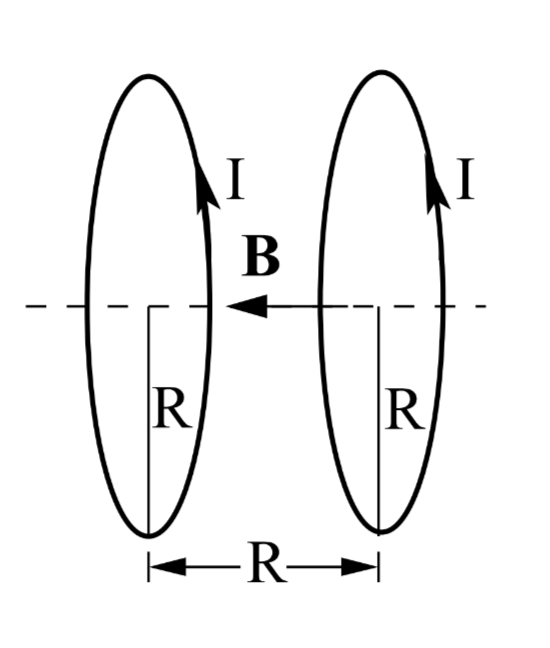
\includegraphics{Bilder/Helmholtz.png}
    \label{fig:helm}
\end{figure}
\noindent Die Berechnung des Magnetfeldes erfolgt dann mithilfe des Biot-Savart-Gesetzes \ref{eqn:Biot} und beträgt für den 
Mittlepunkt des Spulenpaares
\begin{equation}
    \vec{B}(x)=\frac{\mu_0IN}{2}\frac{R^2}{(R^2+x^2)^\frac{3}{2}}\vec{e}_x
    \label{eqn:magfeld}
\end{equation}
insofern die Verbindungsachse als $x$-Achse betrachtet wird. \\

\noindent Das Drehmoment $\vec{M}$ wird im allgemeinen als die Änderungsrate des Drehimpulses $\vec{L}$ in der Zeit beschrieben
\begin{equation}
    \vec{M}=\dot{\vec{L}}\text{ ,}
\end{equation}
wobei der Drehimpuls eines ausgedehnten Körpers über sein Trägheitsmoment 
\begin{equation}
    J_{ij}=\int_V\rho(r)(r^2\delta_{ij}-x_ix_j)\symup{d}V
\end{equation}
beschrieben wird mit 
\begin{equation}
    \vec{L}=\underline{\underline{J}}\vec{\omega} \text{ ,}
    \label{eqn:Drehimpuls}
\end{equation}
wobei dieses für eine Kugel so
\begin{equation}
    J_K=\frac{2}{5}mR^2
    \label{eqn:trägheit_kugel}
\end{equation}
aussieht. \\

\noindent Mit Gleichung \ref{eqn:MagDreh} lässt sich die Differentialgleichung
\begin{equation}
    \vec{m}\times\vec{B}=\frac{\symup{d}\vec{L}}{\symup{d}t}
    \label{eqn:dgl}
\end{equation}
ausschreiben.
Aus dem Betrag von Gleichung \ref{eqn:dgl} folgt für magnetisierte Kugeln, dass
\begin{equation}
    -|\vec{m}\times\vec{B}|=J_K\frac{\symup{d}^2\theta}{\symup{d}t^2}
    \label{eqn:dglmagmom}
\end{equation}
gilt,woraus folgt, dass die Schwingungsdauer sich schreiben lässt als
\begin{equation}
    \frac{1}{T}=\frac{|\vec{m}|}{2\pi L_K}B
    \label{eqn:schwingdauer1}
\end{equation}
beziehungsweise mit $\omega=\frac{2\pi}{T}$ und Gleichung \ref{Drehimpuls} als
\begin{equation}
    T^2=\frac{4\pi^2J_K}{|\vec{m}|}\frac{1}{B} \text{ .}
    \label{eqn:schwingdauer2}
\end{equation}\\

\noindent Steht ein Objekt unter Einfluss der Gravitation, so lässt sich GLeichung \ref{eqn:MagDreh} umschreiben zu
\begin{equation}
    |\vec{m}||\vec{B}|=mdg
    \label{eqn:dreh_grav}
\end{equation}
insofern die Gravitation parallel zum Magnetfeld gerichtet ist.

